\subsection{Technical Review}~\label{technical}

As already breifly introduced, each model was trained for 10,000 iteration steps, covering both the coarse and refine stages or geometry and appearance stages. Notably, the high RAM setting in Colab was enabled, primarily due to the substantial resource demands of Wonder3D. Even with this configuration, there were instances where the training process could be interrupted. Additionally, most of the settings were maintained as per the default Threestudio implementation, although there may have been some minor variations among the methods (some of these can bee seen in Appendix~\ref{ch:differences}). The reason for sticking to these default settings was primarily because altering them might have caused interruptions during training. Moreover, even with the preset configurations, the GPU RAM available on a T4 was often operating close to its maximum capacity.

The rendering time for each method was notably lengthy compared to 2D generative models, which can produce outputs in mere seconds, even with modest computational resources. Detailed information on the training times required for each method, along with various prompts, can be found in Table~\ref{table:generation_times_complex}.

\begin{table}[ht]
    \centering
    \small 
    \begin{tabular}{lcccccccc}
    \toprule
    Prompt & DreamFusion & \multicolumn{2}{c}{Magic3D} & \multicolumn{2}{c}{Fantasia3D} & \multicolumn{2}{c}{Magic123} & Wonder3D \\
    \cmidrule(r){3-4} \cmidrule(lr){5-6} \cmidrule(l){7-8}
    & & \multicolumn{1}{c}{Coarse} & \multicolumn{1}{c}{Refine} & \multicolumn{1}{c}{Geom.} & \multicolumn{1}{c}{Appear.} & \multicolumn{1}{c}{C.} & \multicolumn{1}{c}{R.} &  \\
    \midrule
    Robot & 1:24 & 1:23 & 1:20 & 1:15 & 1:18 & 1:46 & 1:47 & 0:17 \\
    Playmobil & 1:17 & 1:17 & 1:18 & 1:14 & 1:17 & 1:46 & 1:46 & 0:15 \\
    Fern & 1:25 & 1:24 & 1:19 & 1:17 & 1:20 & 1:52 & 1:48 & 0:16 \\
    Bread & 1:25 & 1:21 & 1:21 & 1:17 & 1:20 & 1:54 & 1:52 & 0:15 \\
    \bottomrule
    \end{tabular}
    \caption{Comparison of Generation Times for Different Prompts Across Methods (Hours:Minutes). Legend: C = Coarse, R = Refine, Geom = Geometry, Appear = Appearance.}~\label{table:generation_times_complex}
\end{table}

Among the methods, Wonder3D exhibited the most efficient performance, completing its training in approximately 15 minutes for 10,000 iterations. This is followed by Dreamfusion, which took about 1 hour and 15 minutes to 1 hour and 30 minutes. Magic3D and Fantasia3D demonstrated similar training times of around 1 hour and 15 minutes to 1 hour and 30 minutes each. However, it's worth noting that these two methods involve a two-staged process, resulting in a total training time of approximately 2.5 to 3 hours. The longest training duration was associated with Magic123, requiring approximately 1 hour and 45 minutes to 1 hour and 55 minutes for each coarse and refine stage, summing up to around 3.5 to 3 hours and 50 minutes for 10,000 iteration steps. 
Considering these timeframes within the context of high-performance computing, which encompasses the use of superior and multiple GPUs operating simultaneously, leads to a notable reduction in training duration.

For reference, the setup used in the official papers is as follows:

\begin{itemize}
    \item Dreamfusion: Utilized a single TPUv4, underwent 15,000 iterations, and completed training within 1.5 hours.
    
    \item Fantasia3D\@: Utilized 8 Nvidia RTX 3090 GPUs, with approximately 15 minutes needed for the geometry stage and 16 minutes for the appearance stage.
    
    \item Magic3D\@: Employed 8 Nvidia A100 GPUs, involving 5,000 iterations for the coarse stage with 1,024 samples per ray, taking 15 minutes, and 3,000 iterations for the refine stage, requiring 25 minutes.
    
    \item Magic123: Trained on a 32GB V100 GPU, with 5,000 iterations for both the coarse and fine stages. The coarse stage took around 40 minutes, while the refine stage needed approximately 20 minutes on a 32GB V100.
    
    \item Wonder3D\@: The pretraining phase encompassed the LVIS model, which included over 30,000 objects, and underwent 30,000 iterations on 8 Nvidia Tesla A800 GPUs, spanning approximately 3 days. Subsequently, the extraction of meshes from images could be accomplished in only 2 to 3 minutes.
\end{itemize}


The project Evaluate3D was then used in order to assess specific features of a given mesh, including the CLIP-Score and a rough symmetric value. 

OpenAI's CLIP-score is a metric that quantifies the correspondence between an image and a given prompt \citep{radfordCLIP}. This is achieved by encoding both the prompt and the image into high-dimensional vectors within the same embedding space, and then determining the cosine similarity between these vectors. Despite its sophisticated design, this score is not without limitations and at times cannot rival the discerning capabilities of the human eye, occasionally leading to outcomes that may seem counterintuitive.

For convenience and to streamline the evaluation process, portions of the code using this metric have been integrated into Evaluate3D. Using this feature, scores for the Playmobil figures have been computed and are presented in Table~\ref{table:scorePlaymobil}. In an intriguing turn, Magic123 ranks highest when assessed against the original prompt, followed by Fantasia3D, Wonder3D, DreamFusion, and finally, Magic3D. These findings are not entirely in concordance with the subjective analysis provided earlier. However, when the prompt is changed to ``a high-quality rendering of a red Playmobil firefighter'', there is a marked reversal in scores. This suggests that the CLIP-score may exhibit a bias towards the color black in the context of firefighter apparel, as opposed to the more toy-like red. The discrepancies highlighted by the CLIP-score accentuate the need for the development of new, more precise evaluation metrics tailored for assessing the output of 3D generative AI, as there currently exists no standard method that is universally recognized as reliable.

\begin{table}[ht]
    \centering
    \small
    \begin{tabular}{lccccc}
    \toprule
    Prompt & DreamFusion & Magic3D & Fantasia3D & Magic123 & Wonder3D \\
    \midrule
    a Playmobil firefighter & 0.337 & 0.320 & 0.503 & 0.827 & 0.482 \\
    a red Playmobil firefighter & 0.501 & 0.604 & 0 & 0 & 0.216 \\
    \bottomrule
    \end{tabular}
    \caption{CLIP-scores for Playmobil firefighter models based on different prompts.}~\label{table:scorePlaymobil}
\end{table}

To assess the symmetry of 3D models, several steps were performed. First, an optional rotation of the model is applied for a uniform orientation, which is required for all objects created by DreamFusion, Magic3D, Fantasia3D and Magic123. Then, the given object is split along its X-axis into a left and a right part, creating two halves for the symmetry evaluation.

The core functionality is in the evaluation. Here, the process involves mirroring one half of the model and aligning it with the other. A KDTree structure is created from the vertices of the mirrored right part, facilitating efficient nearest neighbor searches. For each vertex in the left part, the KDTree's query method identifies the closest vertex in the mirrored right part. This method returns a tuple, with the first element being an array of distances between corresponding vertices of the two meshes. The symmetry is evaluated on the basis of these distances. The function counts the number of vertices in the left part whose nearest counterpart in the mirrored right part is within a certain tolerance distance, which is set here to 0.02, which corresponds to approximately 1.5\% of the model size. This count is then used to calculate a symmetry score, expressed as a percentage. The score represents the proportion of vertices in the left part that have a symmetric counterpart within the defined tolerance in the mirrored right part, providing a quantitative measure of the two parts' symmetrical alignment.

However, it should be noted that this value is not an absolute measure of symmetry, as the implementation is currently more of a prototype. Instead, it serves as a rough guide to the relative symmetry between two objects. Reducing and increasing the tolerance will greatly alter the results of the symmetry evaluation. To my knowledge, there is no standardized method to effectively compare the symmetry of different 3D models, especially those with a different number of vertices. The challenge arises from the nature of the division and the properties of triangular 3D meshes. The splitting process is an approximation process that avoids the destruction of triangular surfaces and results in a non-uniform edge. This methodological limitation suggests that further research is needed to develop more precise techniques for the quantitative assessment of 3D models, which may lead to more accurate assessments and guidance in the future.

When the models were prompted with ``a highly symmetrical loaf of bread'', the outcomes were generally unsatisfactory. Among the models tested, only Magic3D and Magic123 were able to create objects that were reasonably symmetrical. This observation is confirmed by the scores listed in Table~\ref{table:symmetryScores}. Given the underwhelming performance, it remains unclear if explicitly requesting symmetry in the prompt leads to improved symmetry in the results. To explore this further, a new prompt was introduced: \textbf{``a symmetrical tennis ball''}. This prompt was chosen with the rationale that a tennis ball, inherently symmetrical in nature, might encourage the generation of more geometrically consistent and thus, more meaningfully comparable results. The results derived from this modified prompt are displayed in Table~\ref{table:symmetryScores} and illustrated in Figure~\ref{fig:Ball}. Considering the relatively simple and detail-sparse nature of a ball, each method underwent a training of 3000 iteration steps, uniformly applied across all stages to ensure consistency in the evaluation process.

\begin{figure}[ht]
    \centering
    \small
    \begin{subfigure}[b]{0.18\textwidth}
        \centering
        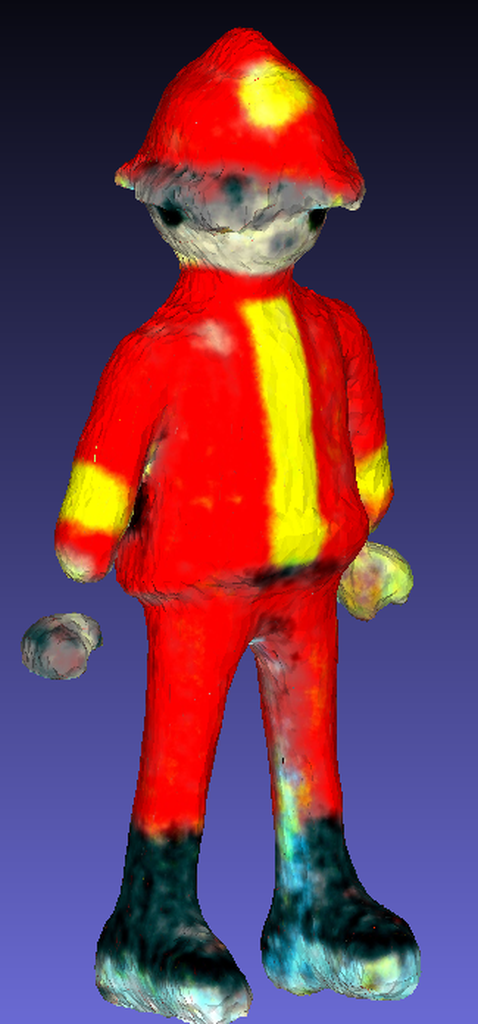
\includegraphics[width=\textwidth]{etc/a high quality rendering of a playmobil firefighter/dreamfusion/dreamfusion_playmobil_result_resize.png}
        \caption{DreamFusion}
    \end{subfigure}
    \begin{subfigure}[b]{0.179\textwidth}
        \centering
        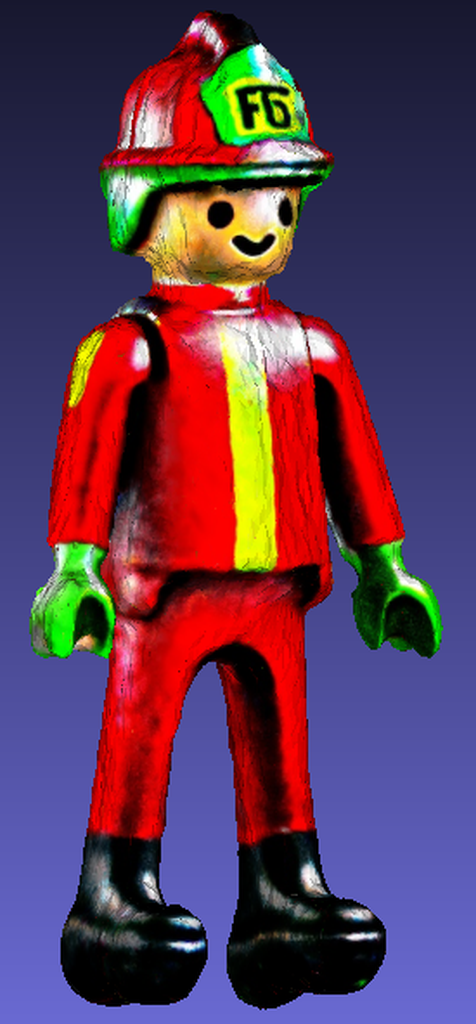
\includegraphics[width=\textwidth]{etc/a high quality rendering of a playmobil firefighter/magic3d/magic3d_playmobil_result_resize.png}
        \caption{Magic3D}
    \end{subfigure}
    \begin{subfigure}[b]{0.227\textwidth}
        \centering
        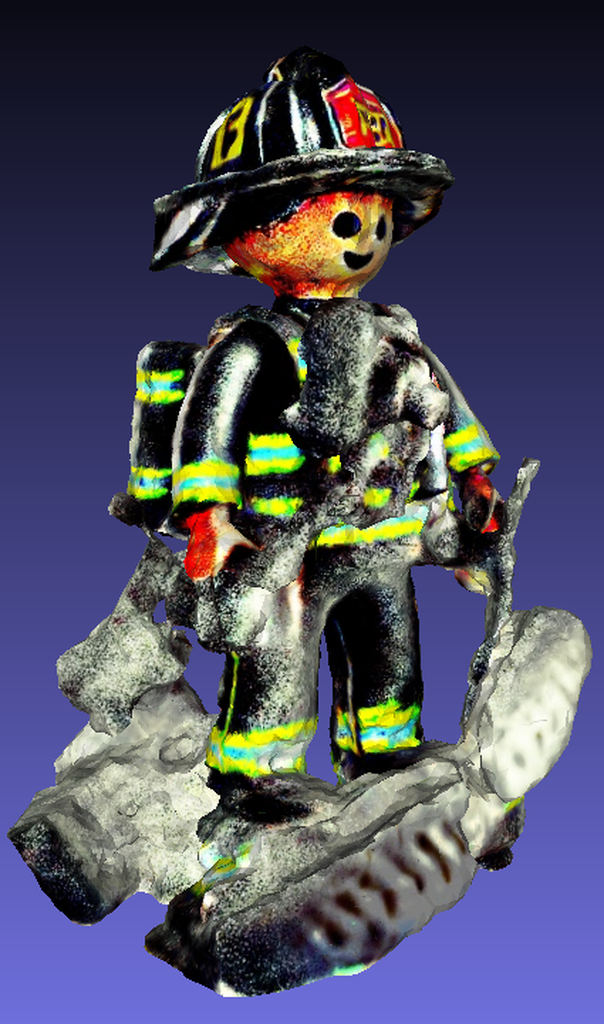
\includegraphics[width=\textwidth]{etc/a high quality rendering of a playmobil firefighter/fantasia3d_Magic3DInput/fantasia_playmobil_result_resize.png}
        \caption{Fantasta3D}
    \end{subfigure}
    \begin{subfigure}[b]{0.192\textwidth}
        \centering
        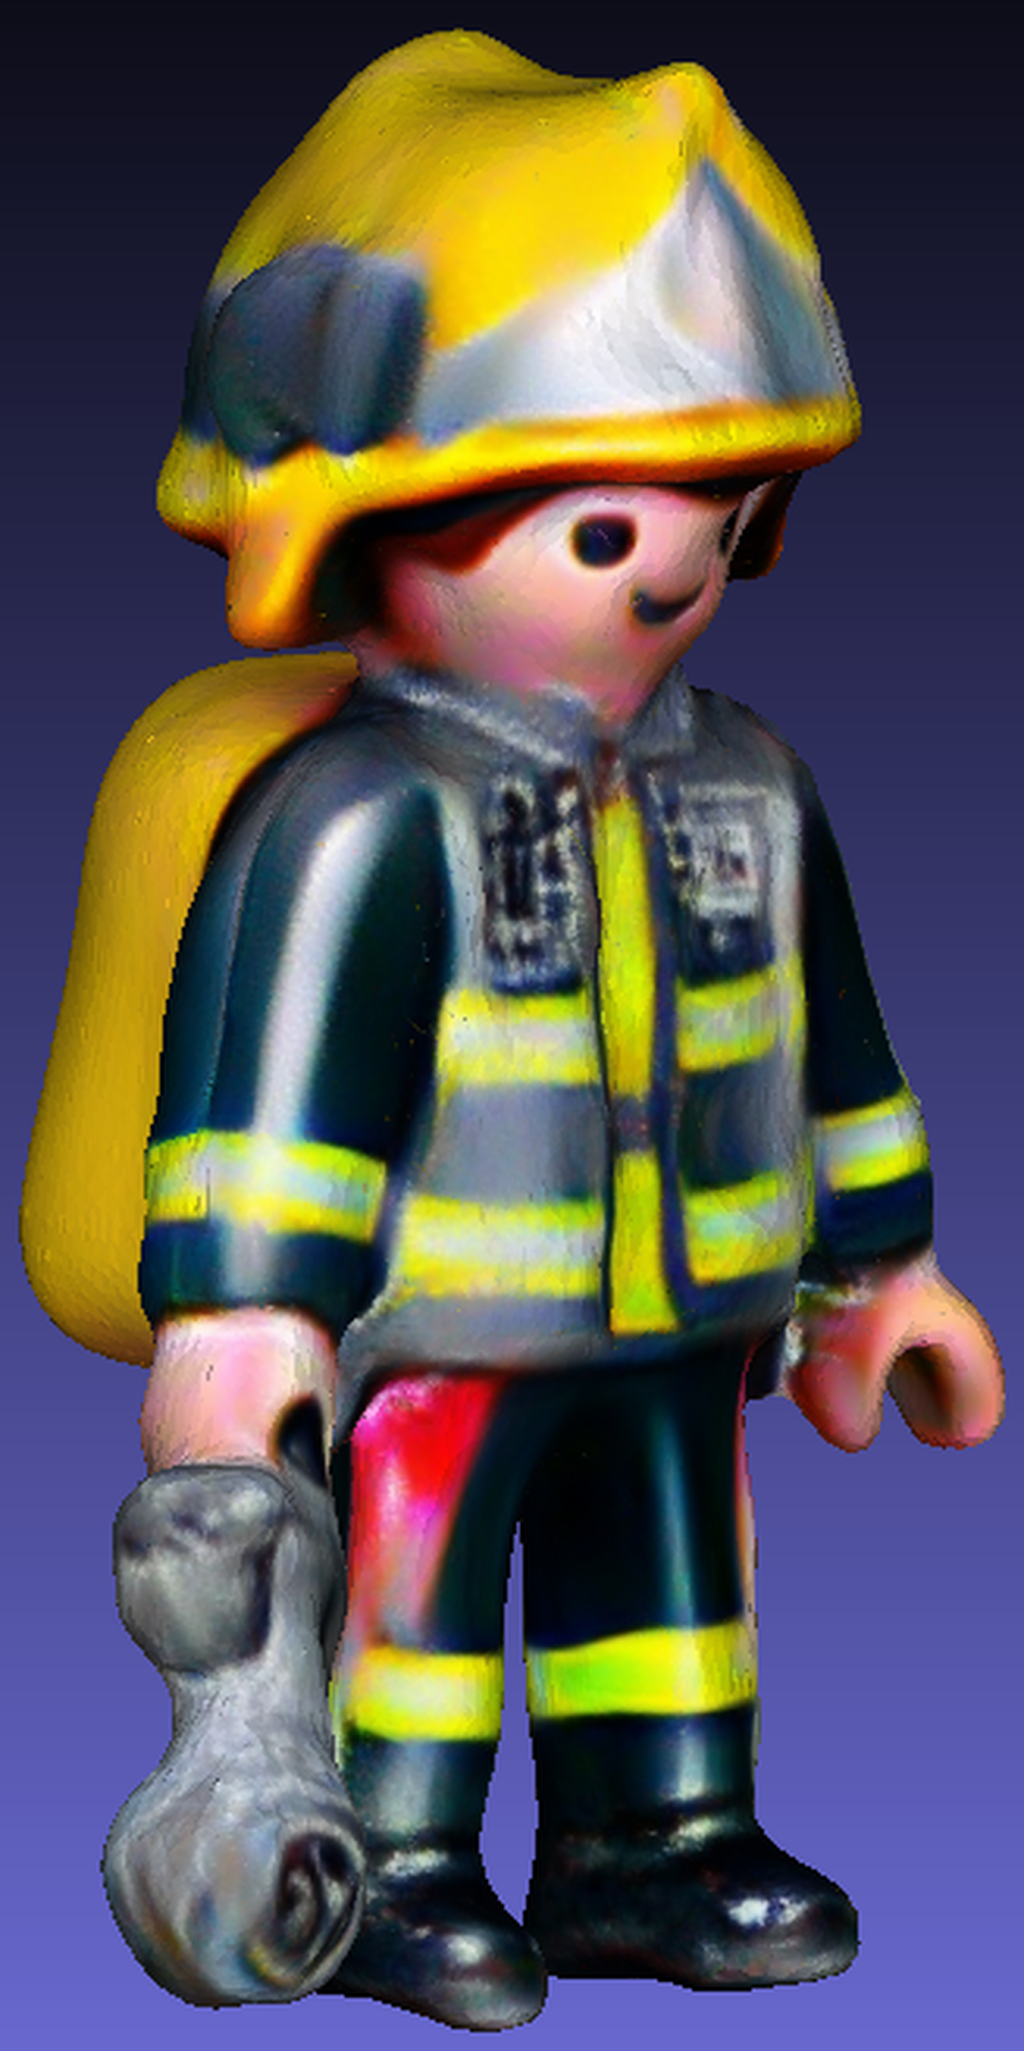
\includegraphics[width=\textwidth]{etc/a high quality rendering of a playmobil firefighter/magic123/magic123_playmobil_result_resize.png}
        \caption{Magic123}
    \end{subfigure}
    \begin{subfigure}[b]{0.181\textwidth}
        \centering
        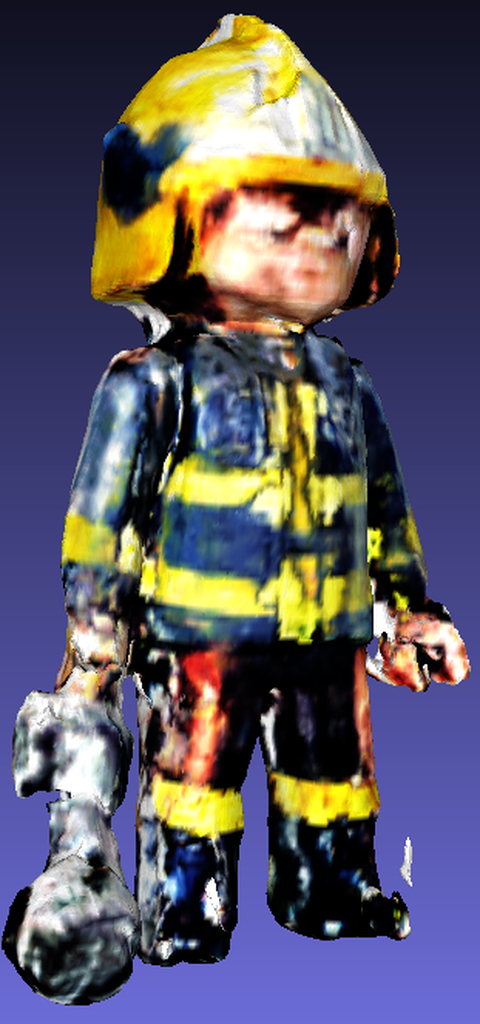
\includegraphics[width=\textwidth]{etc/a high quality rendering of a playmobil firefighter/wonder3D/wonder3d_playmobil_result_resize.png}
        \caption{Wonder3D}
    \end{subfigure}
    \caption{Results obtained using the prompt ``a high-quality rendering of a Playmobil firefighter''.}~\label{fig:Ball}
\end{figure}

\begin{table}[ht]
    \centering
    \small
    \begin{tabular}{lccccc}
    \toprule
    {} & DreamFusion & Magic3D & Fantasia3D & Magic123 & Wonder3D \\
    \midrule
    Loaf of Bread & 0.337 & 0.320 & 0.503 & 0.827 & 0.482 \\
    Tennis Ball & 0.337 & 0.320 & 0.503 & 0.827 & 0.482 \\
    \bottomrule
    \end{tabular}
    \caption{Symmetrie-scores for various prompts demanding a symmetrical output.}~\label{table:symmetryScores}
\end{table}

Based on the new scores, 



